\documentclass{beamer}
\usetheme{Copenhagen}
\usepackage{graphicx}
% \usepackage[ruled,vlined,english]{algorithm2e}
% \renewcommand{\thealgocf}{}
% \usepackage{hyperref}


\author[Jumeau numérique: Environnement]{\large Hanna CHETOUANE, Narmimane ZAOUACHE \\ \vspace{-0.8cm} \date{\today}}
\title[Microclimat urbain]{\textbf{Jumeau numérique dans l'environnement:} \\ Microclimat urbain}



\begin{document}

\begin{frame}
    \titlepage
    \vspace{-0.4cm}
    \begin{center}
        UFR of Mathematics and Informatics - University of Strasbourg 
        \\[0.2cm] 
        \textit{Comment les jumeaux numériques aident-ils à comprendre les effets des aménagements urbains sur le micro-climat ?}
    \end{center}
\end{frame} 


\begin{frame}{Plan}
    \tableofcontents    
\end{frame}


\begin{frame}{Contexte}
    \small
    \begin{itemize} % plus développer ?
        \item L'écologie et le climat sont devenus des enjeux majeurs, surtout dans les villes où se développent des îlots de chaleur
        \item Solutions: Végétalisation, choix de matériaux adaptés et aménagements urbains repensés
        \item Les collectiviités locales doivent ainsi prendre des décisions sur les stratégies d'aménagement à adopter et en évaluer l'impact environnemental et sanitaire
    \end{itemize}
    $\rightarrow$ Simuler et prédire ces effets de ces choix sur le microclimat urbain et la santé publique $\Rightarrow $ \textbf{Jumeau numérique}
\end{frame}


\begin{frame}{Qu'est-ce qu'un jumeau numérique ?}
    \small
    \begin{itemize}
        \item Réplique virtuelle et dynamique d'un système réel, qui, couplé à des outils de simulation, permet d'analyser et prédire son comportement dans différentes conditions
        \item S'appuie sur des données réelles (météorologiques et urbaines) issues de capteurs, d'observations ou de modèles physiques
    \end{itemize}
    \begin{center}
        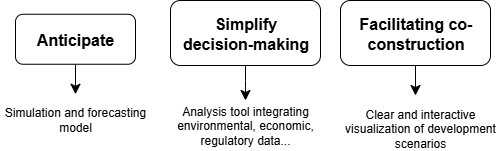
\includegraphics[width=0.7\textwidth]{images/objectifs_jm.png} \\
    \end{center}
    Défi actuel en France: projet JNFT porté par l'IGN, le Cerema et l'Inria, qui vise à créer un jumeau numérique multithématique couvrant le territoire français
\end{frame}


\begin{frame}{Fonctionnement d'un jumeau numérique} %Architecture et pipeline}
    \hspace*{-0.5cm}
    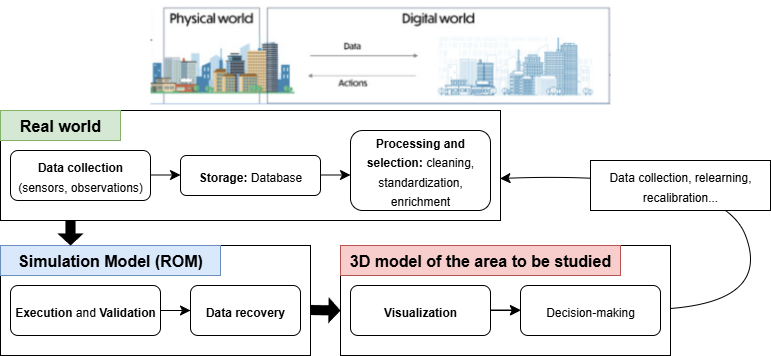
\includegraphics[width=1.1\textwidth]{images/pipeline.png} \\
\end{frame}


\begin{frame}{Méthodes}
    
\end{frame}


\begin{frame}{Données et instrumentation}
    % tableau
\end{frame}


\begin{frame}{Vérification et validation / UQ}
    
\end{frame}


\begin{frame}{Transfert et déploiement}
    
\end{frame}


\begin{frame}{Perspectives et limites}
    
\end{frame}


\begin{frame}{Bibliographie}
    % https://www.ign.fr/institut/un-jumeau-numerique-de-la-france-pour-piloter-la-transition-ecologique
    % https://cnig.gouv.fr/IMG/pdf/2025.01_20_jnft_presentation_cnig_pole_territoires.pdf
    % Fondateurs de la démarche: IGN, Cerema, Inria
    % slide 10 -> 30% pour les aménagements durables
    % https://www.sciencedirect.com/science/article/pii/S2212095525002469
\end{frame}



\end{document}